
%(BEGIN_QUESTION)
% Copyright 2006, Tony R. Kuphaldt, released under the Creative Commons Attribution License (v 1.0)
% This means you may do almost anything with this work of mine, so long as you give me proper credit

Calculate the current through the zener diode for the given values of input (source) voltage in this circuit:

$$\includegraphics[width=15.5cm]{i00757x01.eps}$$

\begin{itemize}
\item{} $V_{source}$ = 25 V ; $I_{zener}$ = 
\item{} $V_{source}$ = 20 V ; $I_{zener}$ = 
\item{} $V_{source}$ = 15 V ; $I_{zener}$ = 
\item{} $V_{source}$ = 10 V ; $I_{zener}$ = 
\item{} $V_{source}$ = 5 V ; $I_{zener}$ = 
\end{itemize}

Do you see any relationship between source voltage and zener diode current?  If so, explain what that relationship is.

\underbar{file i00757}
%(END_QUESTION)





%(BEGIN_ANSWER)

As the source voltage decreases, zener diode current also decreases:

\begin{itemize}
\item{} $V_{source}$ = 25 V ; $I_{zener}$ = 41.49 mA
\item{} $V_{source}$ = 20 V ; $I_{zener}$ = 30.85 mA
\item{} $V_{source}$ = 15 V ; $I_{zener}$ = 20.21 mA
\item{} $V_{source}$ = 10 V ; $I_{zener}$ = 9.58 mA
\item{} $V_{source}$ = 5 V ; $I_{zener}$ = 0 mA
\end{itemize}

It should be noted that the calculated answers shown here will {\it not} precisely match a real zener diode circuit, due to the fact that zener diodes tend to gradually taper off in current as the applied voltage nears the zener voltage rating rather than current sharply dropping to zero as a simpler model would predict.

%(END_ANSWER)





%(BEGIN_NOTES)

This exercise in current calculation is supposed to get students to realize the inverse relationship between input voltage and zener current: that the zener diode regulates voltage by acting as a parasitic load of varying proportion.  Simply put, the diode loads down the circuit as much as needed to maintain a stable voltage at the load terminals.

%INDEX% Electronics review: zener diode voltage regulator circuit

%(END_NOTES)


